% -----------------------------------------------------
% Caption color-key chips for result tables and figures.
% These commands are kept local to the Results section so no preamble edit is required.
% -----------------------------------------------------
\DeclareRobustCommand{\greenhl}[1]{%
  \begingroup\setlength{\fboxsep}{1.2pt}\colorbox{PositiveCell}{\strut #1}\endgroup}
\DeclareRobustCommand{\redhl}[1]{%
  \begingroup\setlength{\fboxsep}{1.2pt}\colorbox{NegativeCell}{\strut #1}\endgroup}
\DeclareRobustCommand{\neutralhl}[1]{%
  \begingroup\setlength{\fboxsep}{1.2pt}\colorbox{NeutralCell}{\strut #1}\endgroup}

\section{Results}
\label{sec:results}

This section reports the experimental results at three levels. We first evaluate cross-task transfer on ACL Bench for Base, DD-LoRA, and RC-LoRA across three open-weight checkpoints. We then examine constraint-induced relative preference shifts using controlled behavioral probes for Qwen2.5-7B. Finally, we analyze how rule-constrained fine-tuning changes the causal contribution of individual attention heads and validate the highest-ranked heads through joint Top-$k$ ablation against two random-control conditions.

\subsection{Task-Transfer Results}
\label{sec:task_transfer_results}

\subsubsection{Overall ACL Bench Performance}

Table~\ref{tab:acl_overall} and Figure~\ref{fig:acl_transfer} report overall ACL Bench accuracy for the three model states. DD-LoRA denotes ordinary mixed-data adaptation, whereas RC-LoRA denotes the constraint-enriched condition.

\begin{table}[H]
\centering
\caption{Overall ACL Bench accuracy for Base, DD-LoRA, and RC-LoRA. Values are percentages. $\Delta_{\mathrm{RC-DD}}$ is the RC-LoRA minus DD-LoRA difference in percentage points. \greenhl{Green-toned} highlighting marks positive RC-LoRA-over-DD-LoRA changes; unshaded black text is neutral.}
\label{tab:acl_overall}
\vspace{0.45em}
\begin{tabular}{lrrrr}
\toprule
\rowcolor{NeutralCell}
Model & Base & DD-LoRA & RC-LoRA & $\Delta_{\mathrm{RC-DD}}$ \\
\midrule
DeepSeek-R1-\allowbreak Distill-\allowbreak Llama-8B & 28.3 & 31.7 & 38.0 & \poscell{+6.3} \\
Qwen2.5-7B                  & 35.3 & 54.0 & 58.7 & \poscell{+4.7} \\
Llama3.1-8B                 & 45.0 & 42.3 & 46.7 & \poscell{+4.4} \\
\bottomrule
\end{tabular}
\end{table}

The ordinary DD-LoRA condition is strongly model-dependent. DeepSeek-R1-Distill-Llama-8B increases from 28.3\% to 31.7\%, and Qwen2.5-7B increases from 35.3\% to 54.0\%, whereas Llama3.1-8B decreases from 45.0\% to 42.3\%. Thus, ordinary mixed-data fine-tuning can produce substantial positive transfer for some checkpoints while inducing mild negative transfer for another.

RC-LoRA achieves 38.0\%, 58.7\%, and 46.7\% on DeepSeek-R1-Distill-Llama-8B, Qwen2.5-7B, and Llama3.1-8B, respectively. Relative to DD-LoRA, the corresponding overall changes are +6.3, +4.7, and +4.4 percentage points. Relative to Base, the RC-LoRA changes are +9.7, +23.4, and +1.7 percentage points. The consistent RC-LoRA-over-DD-LoRA direction across all three checkpoints indicates a more consistently positive transfer profile for the constraint-enriched regime than for the ordinary mixed-data regime. Figure~\ref{fig:acl_transfer} visualizes the three-way overall comparison and makes the DD-to-RC increment explicit for each checkpoint.

\begin{figure}[ht]
\centering
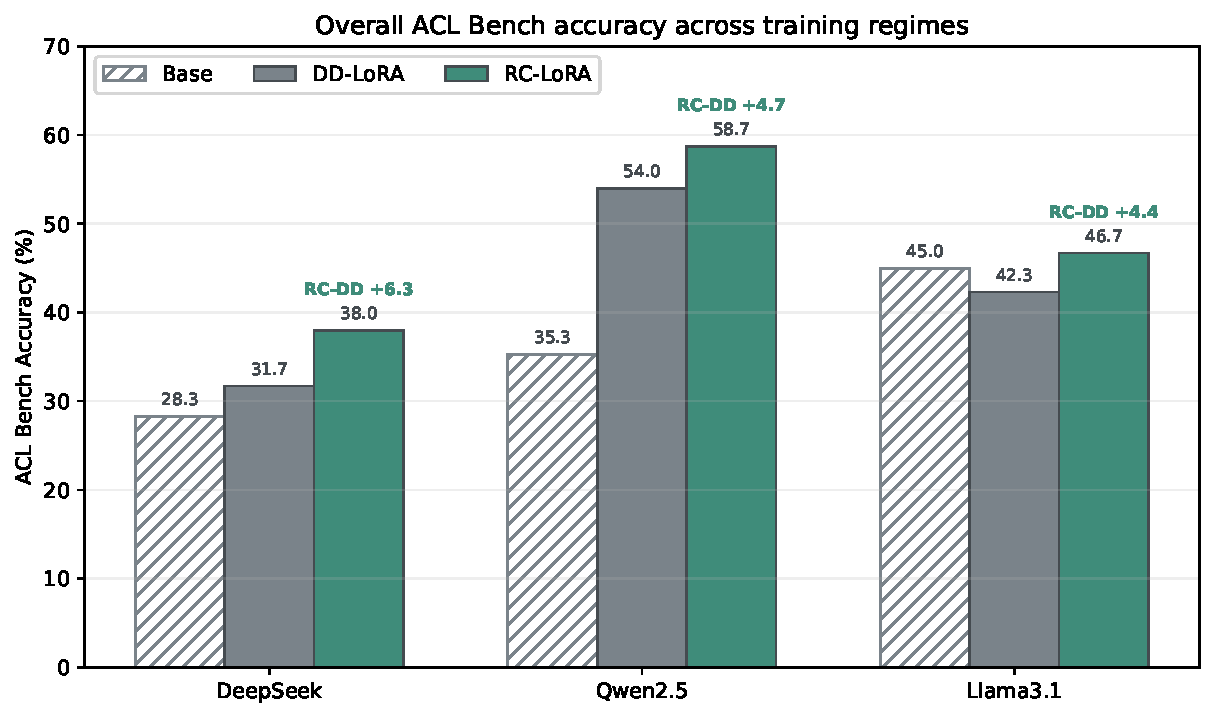
\includegraphics[width=0.86\linewidth]{figures/figure6_acl_transfer.pdf}
\caption{
Overall ACL Bench accuracy for Base, DD-LoRA, and RC-LoRA across the three evaluated checkpoints. The annotations above the RC-LoRA bars show the RC-LoRA minus DD-LoRA increment in percentage points. \greenhl{Green-toned} elements emphasize the focal RC-LoRA condition and its positive increment, whereas \neutralhl{gray/black or unfilled} elements denote neutral comparison states.
}
\label{fig:acl_transfer}
\end{figure}

\subsubsection{Category-Level Transfer}

Table~\ref{tab:acl_categories} reports category-level accuracy for Base, DD-LoRA, and RC-LoRA, while Figure~\ref{fig:acl_category_transfer} summarizes the corresponding Base-to-DD-LoRA and DD-LoRA-to-RC-LoRA changes.

\begin{table}[H]
\centering
\caption{Category-level ACL Bench accuracy for Base, DD-LoRA, and RC-LoRA. Values are percentages. \greenhl{Green-toned} RC-LoRA cells are higher than the corresponding DD-LoRA values; unshaded black entries are neutral.}
\label{tab:acl_categories}
\vspace{0.45em}
\begin{tabular}{llrrr}
\toprule
\rowcolor{NeutralCell}
Model & Setting & Counter & Hierarchy & Pattern \\
\midrule
DeepSeek & Base    & 24 & 35 & 26 \\
         & DD-LoRA & 28 & 30 & 37 \\
         & RC-LoRA & \poscell{37} & \poscell{40} & 37 \\
\midrule
Qwen2.5 & Base    & 34 & 36 & 36 \\
        & DD-LoRA & 39 & 60 & 63 \\
        & RC-LoRA & \poscell{46} & \poscell{65} & \poscell{65} \\
\midrule
Llama3.1 & Base    & 34 & 58 & 43 \\
         & DD-LoRA & 30 & 51 & 46 \\
         & RC-LoRA & 30 & \poscell{58} & \poscell{52} \\
\bottomrule
\end{tabular}
\end{table}

The DD-LoRA results already show selective transfer. For DeepSeek, Pattern Recognition improves from 26\% to 37\%, while Hierarchy Logic decreases from 35\% to 30\%. Qwen2.5 improves in all three categories, most strongly in Hierarchy Logic (36\% to 60\%) and Pattern Recognition (36\% to 63\%). Llama3.1 shows a smaller Pattern Recognition gain (43\% to 46\%) but decreases on Counter Logic and Hierarchy Logic.

Adding the constraint-enriched training regime produces a non-negative DD-LoRA-to-RC-LoRA change in every reported category. DeepSeek gains +9 points on Counter Logic and +10 on Hierarchy Logic while remaining unchanged on Pattern Recognition. Qwen2.5 gains +7, +5, and +2 points on Counter Logic, Hierarchy Logic, and Pattern Recognition, respectively. Llama3.1 remains unchanged on Counter Logic but gains +7 on Hierarchy Logic and +6 on Pattern Recognition.

These results support two distinctions. First, structural transfer is not introduced only by the constraint examples: ordinary DD-LoRA already produces large gains for some model--category pairs, particularly Qwen2.5 Hierarchy Logic and Pattern Recognition. Second, the constraint-enriched RC-LoRA condition is associated with a consistent positive overall increment relative to DD-LoRA and with non-negative category-level changes across the three evaluated checkpoints. The effect is therefore better characterized as selective and model-dependent transfer with an additional cross-checkpoint consistency in the RC-LoRA-over-DD-LoRA direction, rather than as a uniform increase in general reasoning ability. Figure~\ref{fig:acl_category_transfer} separates the two transition stages visually: the left panel shows Base $\rightarrow$ DD-LoRA changes, and the right panel shows the additional DD-LoRA $\rightarrow$ RC-LoRA changes.

\begin{figure}[ht]
\centering
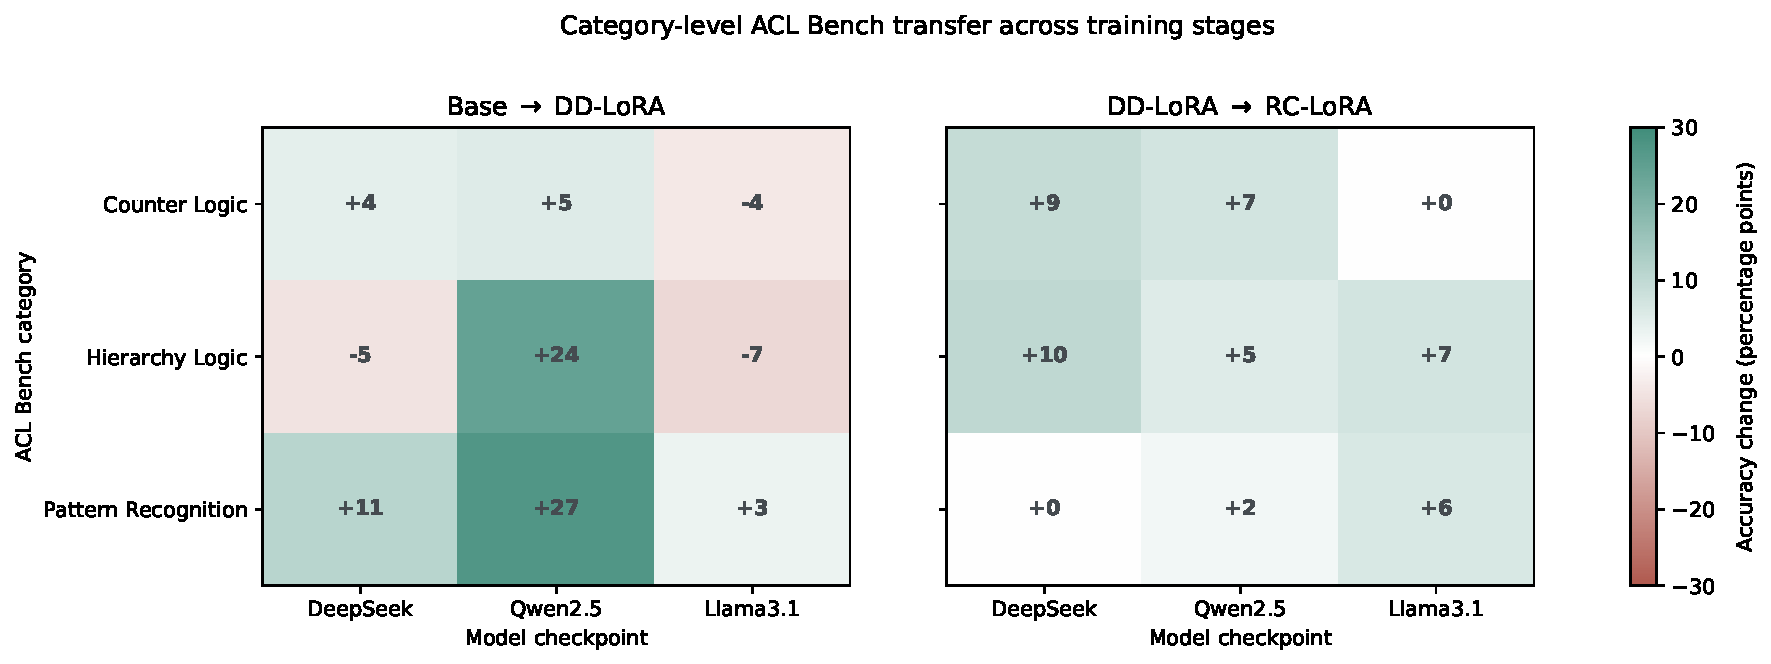
\includegraphics[width=0.96\linewidth]{figures/figure7_acl_category_transfer.pdf}
\caption{
Category-level ACL Bench transfer across training stages. Left: Base-to-DD-LoRA accuracy changes. Right: DD-LoRA-to-RC-LoRA accuracy changes. \greenhl{Green-toned} cells indicate positive accuracy changes, \redhl{red-toned} cells indicate negative changes, and \neutralhl{neutral-toned} cells indicate values near zero.
}
\label{fig:acl_category_transfer}
\end{figure}

\subsection{Constraint-Sensitive Preference-Shift Results}
\label{sec:constraint_behavior_results}

ACL Bench evaluates transfer outside the source domain, but it does not directly measure whether the fine-tuned model has learned to revise its decision preference when an additional rule prohibits an otherwise preferred action. We therefore evaluate Qwen2.5-7B Base and RC-LoRA on the 60 controlled constraint-sensitive probes using BCDM.

\subsubsection{Overall Relative-Preference Shift}

Table~\ref{tab:constraint_overall} summarizes the overall preference-shift scores.

\begin{table}[t]
\centering
\caption{BCDM on the 60 constraint-sensitive probes. Values are reported as mean $\pm$ standard deviation. \greenhl{Green-toned} highlighting marks the higher BCDM relative-preference-shift score compared with Base; unshaded black entries are neutral.}
\label{tab:constraint_overall}
\vspace{0.45em}
\begin{tabular}{lc}
\toprule
\rowcolor{NeutralCell}
Model & BCDM \\
\midrule
Qwen2.5-7B Base & $1.391 \pm 1.379$ \\
Qwen2.5-7B RC-LoRA & \poscell{$4.371 \pm 0.766$} \\
\bottomrule
\end{tabular}
\end{table}

Mean BCDM increases from $1.391 \pm 1.379$ for the Base model to $4.371 \pm 0.766$ for RC-LoRA, a gain of approximately 2.981 points. Because BCDM measures the change in the relative log-probability margin between the forbidden action and the strongest legal alternative, the increase indicates a larger constraint-induced relative preference shift in RC-LoRA. The relatively large standard deviation of the Base model is consistent with the heterogeneous scenario-level behavior reported below: several scenarios produce small mean shifts, whereas \path{straight_34567} already produces a much larger Base response. The aggregate Base score therefore combines probes with substantially different levels of constraint sensitivity rather than reflecting a uniformly distributed response, while RC-LoRA shows a smaller standard deviation and a more consistent BCDM response across the evaluated probes. Importantly, BCDM should not be interpreted as final-action compliance: a positive BCDM can coexist with the forbidden action remaining the highest-probability output, so the metric does not by itself indicate that a legal alternative becomes the generated action.

\subsubsection{Scenario-Level Results}

The 60 probes are divided equally across six controlled scenarios, with 10 probes per scenario. Table~\ref{tab:constraint_scenarios} reports the corresponding mean scores.

\begin{table}[t]
\centering
\caption{Scenario-level BCDM for Qwen2.5-7B. Each scenario contains 10 probes. \greenhl{Green-toned} $\Delta$ values indicate larger BCDM after fine-tuning, \redhl{red-toned} values indicate a decline, and unshaded black entries are neutral references.}
\label{tab:constraint_scenarios}
\vspace{0.45em}
\begin{tabular}{lrrr}
\toprule
\rowcolor{NeutralCell}
Scenario & Base & RC-LoRA & $\Delta$ \\
\midrule
\path{bomb_9999}              & 1.898 & 4.180 & \poscell{+2.282} \\
\path{pair_88}                & 0.309 & 5.284 & \poscell{+4.975} \\
\path{real_pair_QQ_landlord}& 0.155 & 4.107 & \poscell{+3.952} \\
\path{rocket_BR}              & 1.115 & 5.427 & \poscell{+4.312} \\
\path{single_A_follow}       & 0.700 & 3.252 & \poscell{+2.552} \\
\path{straight_34567}         & 4.168 & 3.977 & \negcell{-0.191} \\
\bottomrule
\end{tabular}
\end{table}

RC-LoRA achieves a higher constraint-sensitive score in five of the six scenarios, with the largest gains of 4.975 for \path{pair_88}, 4.312 for \path{rocket_BR}, and 3.952 for \path{real_pair_QQ_landlord}. The \path{straight_34567} scenario differs from the others: the Base model already exhibits a relatively high score of 4.168, while the RC-LoRA score is slightly lower at 3.977. The fine-tuning effect is therefore not uniformly positive across every individual scenario. Nevertheless, the overall mean increases substantially, and five of the six scenario-level comparisons show a larger BCDM for RC-LoRA. These results support a cross-scenario increase in the measured constraint-induced relative preference shift while also indicating that the magnitude of the effect depends on the underlying decision structure.

\begin{figure}[ht]
\centering
\resizebox{0.98\linewidth}{!}{%
\begin{tikzpicture}[x=1cm,y=0.78cm]

% Plot area
\def\xmax{10.5}
\def\ymax{6}

% Horizontal grid and y-axis ticks
\foreach \y in {0,1,2,3,4,5,6} {
    \draw[draw=Ink!14,line width=0.35pt] (0,\y) -- (\xmax,\y);
    \node[font=\scriptsize,anchor=east,text=Ink!75] at (-0.18,\y) {\y};
}

% Axes
\draw[draw=Ink!70,line width=0.7pt] (0,0) -- (\xmax,0);
\draw[draw=Ink!70,line width=0.7pt] (0,0) -- (0,\ymax);

% Axis labels
\node[font=\small,rotate=90,text=Ink!90] at (-0.85,3) {Mean BCDM};
\node[font=\small,text=Ink!90] at (5.25,-2.05) {Scenario};

% X-axis scenario labels
\node[font=\scriptsize\ttfamily,align=center,anchor=north,text=Ink!80]
    at (0, -0.24) {bomb\\9999};
\node[font=\scriptsize\ttfamily,align=center,anchor=north,text=Ink!80]
    at (2.1, -0.24) {pair\\88};
\node[font=\scriptsize\ttfamily,align=center,anchor=north,text=Ink!80]
    at (4.2, -0.24) {real\_pair\\QQ landlord};
\node[font=\scriptsize\ttfamily,align=center,anchor=north,text=Ink!80]
    at (6.3, -0.24) {rocket\\BR};
\node[font=\scriptsize\ttfamily,align=center,anchor=north,text=Ink!80]
    at (8.4, -0.24) {single\_A\\follow};
\node[font=\scriptsize\ttfamily,align=center,anchor=north,text=Ink!80]
    at (10.5, -0.24) {straight\\34567};

% Base: dashed line for grayscale readability
\draw[draw=Ink!72,line width=1.25pt,dashed]
    (0,1.898) --
    (2.1,0.309) --
    (4.2,0.155) --
    (6.3,1.115) --
    (8.4,0.700) --
    (10.5,4.168);

% RC-LoRA: solid line
\draw[draw=Positive!90,line width=1.55pt]
    (0,4.180) --
    (2.1,5.284) --
    (4.2,4.107) --
    (6.3,5.427) --
    (8.4,3.252) --
    (10.5,3.977);

% Data-point markers
\foreach \x/\y in {0/1.898,2.1/0.309,4.2/0.155,6.3/1.115,8.4/0.700,10.5/4.168} {
    \fill[Ink!72] (\x,\y) circle (2.2pt);
}
\foreach \x/\y in {0/4.180,2.1/5.284,4.2/4.107,6.3/5.427,8.4/3.252,10.5/3.977} {
    \fill[Positive!90] (\x,\y) circle (2.5pt);
}

% Legend placed above the plotting area so it never covers the data lines
\draw[draw=Ink!18,fill=white,line width=0.35pt] (6.85,6.22) rectangle (10.45,7.42);

\draw[draw=Ink!72,line width=1.25pt,dashed] (7.15,7.06) -- (7.90,7.06);
\fill[Ink!72] (7.53,7.06) circle (2.2pt);
\node[font=\small,anchor=west,text=Ink!90] at (8.35,7.06) {Base};

\draw[draw=Positive!90,line width=1.55pt] (7.15,6.60) -- (7.90,6.60);
\fill[Positive!90] (7.53,6.60) circle (2.5pt);
\node[font=\small,anchor=west,text=Ink!90] at (8.35,6.60) {RC-LoRA};

\end{tikzpicture}%
}

\caption{
Scenario-level BCDM for Qwen2.5-7B Base and RC-LoRA across six constraint-sensitive scenarios. Each point is the mean over 10 probes. The \greenhl{green-toned} line denotes the focal RC-LoRA condition, while the \neutralhl{black/gray} line is the neutral Base reference; scenario-wise improvement or decline is determined by their relative heights.
}
\label{fig:preference_shift}
\end{figure}

\subsubsection{Preference--Generation Gap}

The larger probability-level relative shift does not translate into better greedy-decoding compliance. Under direct generation, the Base model selects the forbidden action in 40 of 60 probes (66.7\%) and a legal action in the remaining 20 probes; 10 of these legal outputs match the designated allowed action and 10 are other legal alternatives. RC-LoRA selects the forbidden action in all 60 probes. Thus, the legal-action rate decreases from 33.3\% for Base to 0\% for RC-LoRA.

This diagnostic establishes a clear separation between the BCDM-based relative preference shift and executable compliance. The current results do not show improved rule-compliant generation after RC-LoRA; instead, they show that the constraint produces a larger change in the relative legal-versus-forbidden margin even though the forbidden action still wins under greedy decoding. The mechanistic analyses below therefore concern the probability-level effect measured by BCDM, not final-action compliance.


\subsection{Attention-Head Causal Results}
\label{sec:head_causal_results}

RC-LoRA shows a substantially larger BCDM than the Base model. We next examine whether this Base-to-RC difference is accompanied by changes in the functional importance of individual attention heads, focusing the causal analysis on Qwen2.5-7B.

\subsubsection{Exploratory Attention-Based Screening}

Before performing the complete intervention scan, we explored whether constraint-related attention heads could be identified through a three-stage attention-based screening procedure consisting of targeting, correlation, and counterfactual filtering. For the Base model, the screening sequence was $784\rightarrow157\rightarrow22\rightarrow14$ candidate heads. The standard RC-LoRA sequence was $784\rightarrow157\rightarrow0\rightarrow0$. Under a relaxed RC-LoRA setting using 100 samples, the targeting stage retained 235 heads, but none survived the subsequent correlation stage ($784\rightarrow235\rightarrow0\rightarrow0$). These results indicate that simple attention--behavior correlation does not provide a stable basis for identifying constraint-relevant components after fine-tuning; rather than treating the absence of correlated heads as evidence that the model lacks localized functional dependence, we therefore proceed to direct causal intervention.

\subsubsection{Complete Single-Head Causal Scan}

Qwen2.5-7B contains 28 Transformer layers with 28 attention heads per layer, yielding 784 heads in total. Each head is independently ablated in both the Base and RC-LoRA models, producing 1,568 single-head interventions. For every intervention, we compute the causal contribution and the Base-to-RC-LoRA change $\Delta CE(l,h)$ defined in Eq.~\ref{eq:delta_ce}. The resulting distribution is highly heterogeneous: most heads show relatively small causal changes, while a much smaller subset exhibits substantially larger positive $\Delta CE$ values.

\begin{figure}[t]
\centering
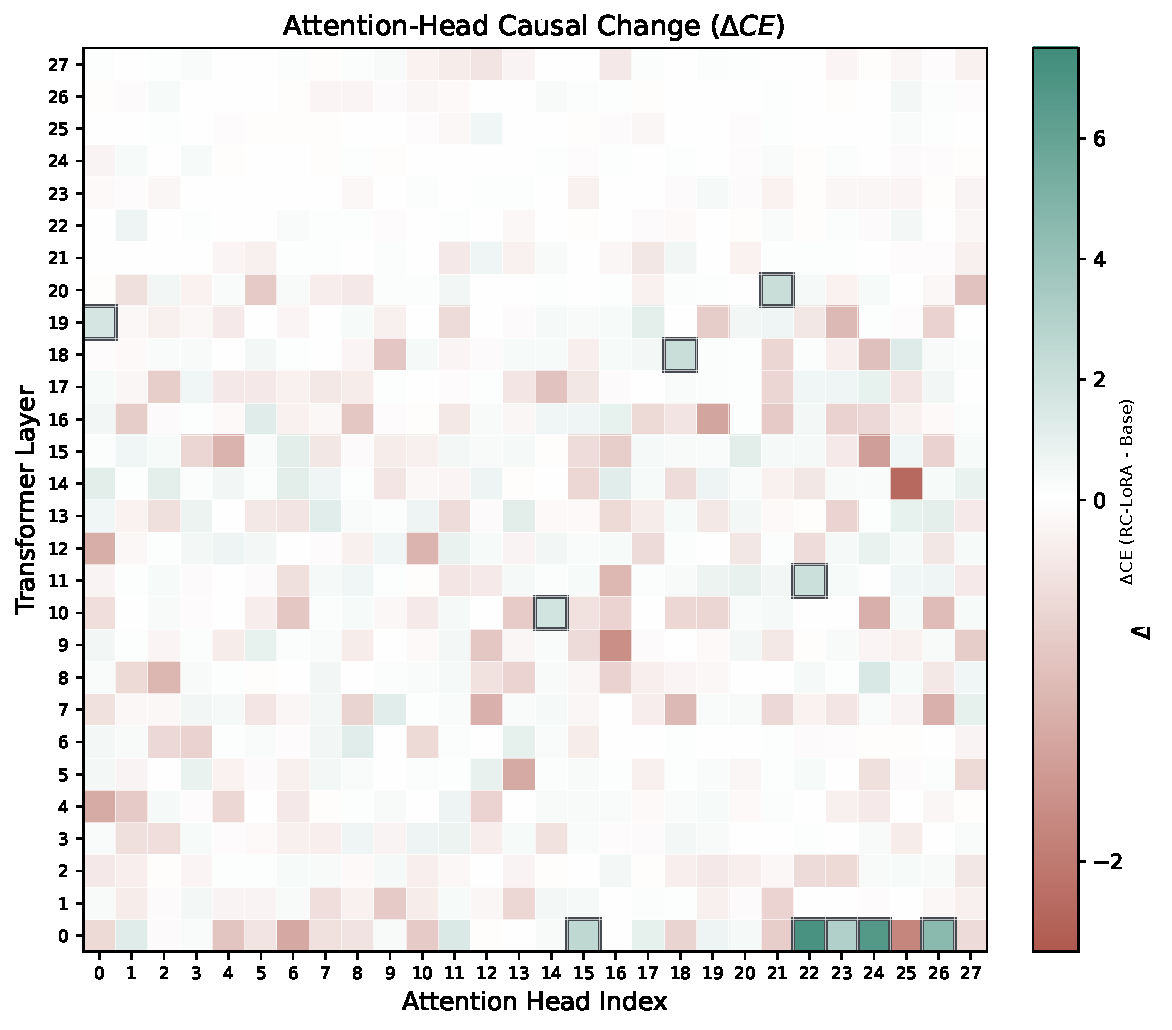
\includegraphics[width=0.78\linewidth]{figures/figure_attention_head_heatmap.pdf}
\caption{
Attention-head heatmap of Base-to-RC-LoRA causal change $\Delta CE$ for Qwen2.5-7B.
Rows correspond to Transformer layers and columns correspond to attention-head indices.
\greenhl{Green-toned} hues indicate $\Delta CE>0$, \redhl{red-toned} hues indicate $\Delta CE<0$, and near-neutral tones indicate values close to zero. \neutralhl{Black} outlines are neutral markers that identify the ten heads with the largest positive causal changes.
The distribution shows sparse and heterogeneous redistribution of causal dependence across attention heads.
}
\label{fig:attention_heatmap}
\end{figure}

Negative values are also observed, indicating that some heads become less supportive of the measured behavior after fine-tuning or that their removal improves the preference-shift score. Together, the positive and negative changes show that causal dependence is redistributed non-uniformly rather than uniformly strengthened across the attention system. Figure~\ref{fig:layerwise_delta_ce} summarizes the positive component of this redistribution across Transformer layers.

\begin{figure}[!tbp]

\centering

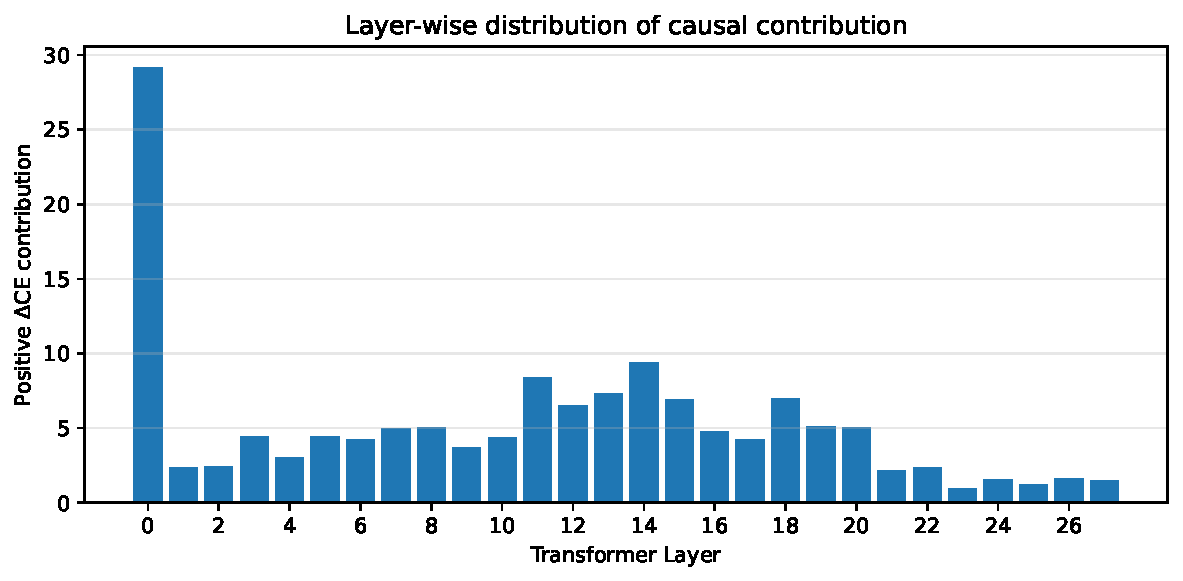
\includegraphics[
width=0.85\linewidth
]{figures/figure8_layerwise_delta_ce.pdf}

\caption{
Layer-wise distribution of positive causal contribution measured by $\Delta CE$ across Qwen2.5-7B attention heads. The \greenhl{green-toned} bars represent positive causal-change contributions, while black/gray axes and grid elements are neutral visual references. The distribution shows non-uniform changes in causal contribution across Transformer layers after fine-tuning.
}

\label{fig:layerwise_delta_ce}

\end{figure}

The layer-wise pattern remains non-uniform, and Table~\ref{tab:top_heads} reports the ten heads with the largest positive $\Delta CE$ values.

\begin{table}[t]
\centering
\caption{Top ten Qwen2.5-7B attention heads ranked by Base-to-RC-LoRA causal change $\Delta CE$. All listed heads exhibit positive $\Delta CE$, indicating higher causal contribution in RC-LoRA than in Base under the present metric.}
\label{tab:top_heads}
\vspace{0.45em}
\begin{tabular}{rrr}
\toprule
\rowcolor{NeutralCell}
Rank & Attention Head & $\Delta CE$ \\
\midrule
1  & L0-H22  & 7.062 \\
2  & L0-H24  & 6.671 \\
3  & L0-H26  & 4.552 \\
4  & L0-H23  & 2.996 \\
5  & L0-H15  & 2.486 \\
6  & L20-H21 & 2.101 \\
7  & L18-H18 & 2.055 \\
8  & L11-H22 & 2.046 \\
9  & L10-H14 & 1.746 \\
10 & L19-H0  & 1.595 \\
\bottomrule
\end{tabular}
\end{table}

Several of the strongest causal changes are concentrated in Layer 0: five of the ten highest-ranked heads are located in the first Transformer layer. However, positive $\Delta CE$ values are not restricted to the earliest layer, with additional top-ranked heads appearing in Layers 10, 11, 18, 19, and 20. The pattern therefore combines strong early-layer concentration with additional high-impact components distributed across intermediate layers, rather than indicating a mechanism confined to a single network depth.

\subsubsection{Representative Head: L0-H22}

L0-H22 provides the clearest example of causal amplification after fine-tuning. In the Base model, ablating this head reduces the preference-shift score from 1.390711 to 0.751787, giving $CE_{\mathrm{Base}}=0.638924$. In RC-LoRA, the same ablation changes the score from 4.371395 to $-3.329531$, giving $CE_{\mathrm{RC\text{-}LoRA}}=7.700926$. The resulting Base-to-RC-LoRA change is therefore $\Delta CE=7.062002$. L0-H22 is thus already positively involved in the measured behavior before fine-tuning, but its causal contribution becomes much larger afterward. This pattern is consistent with selective amplification or functional reconfiguration of an existing component rather than the appearance of an entirely new attention-head function.

\subsubsection{Causal Heterogeneity Across Heads}

The complete scan reveals several qualitatively different patterns of causal change. Some heads satisfy $CE_{\mathrm{RC\text{-}LoRA}}\gg CE_{\mathrm{Base}}>0$, indicating strong amplification of an already positive Base-model contribution, while others have weak Base contributions but become substantially positive after fine-tuning. Many heads remain near $\Delta CE\approx0$, whereas a smaller subset has $\Delta CE<0$, showing that fine-tuning can also reduce the measured contribution of individual components. Together, these results support a sparse and non-uniform redistribution of causal dependence rather than uniform strengthening of attention heads across the network, and they help explain why attention-based correlation alone is insufficient for identifying the relevant components: strong causal importance after fine-tuning does not necessarily correspond to a simple observable attention--behavior correlation.

\subsubsection{Top-k Joint-Ablation Validation}

Single-head causal effects identify components whose individual importance changes after fine-tuning, but they do not establish whether the highest-ranked heads form a collectively important functional subset. We therefore jointly ablate the Top-$k$ heads ranked by $\Delta CE$ for $k\in\{5,10,27\}$ and compare the resulting behavioral degradation against Global Random and Matched Random controls, each averaged over five independently sampled control sets; the comparison is summarized in Figure~\ref{fig:topk_validation}.

\begin{figure}[ht]
\centering

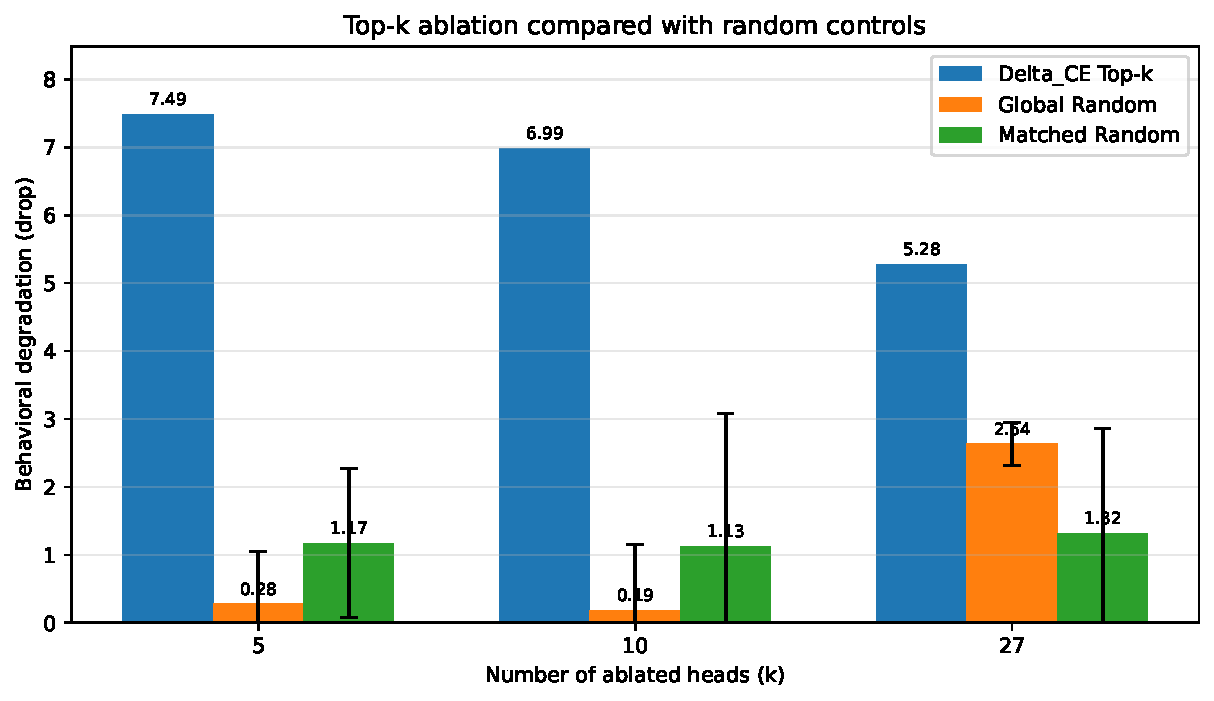
\includegraphics[width=0.65\linewidth]{figures/figure4b_random_controls.pdf}


\vspace{0.2cm}


\begin{minipage}{0.7\linewidth}
\centering
\scriptsize

\begin{tabular}{rrrr}
\toprule
\rowcolor{NeutralCell}
$k$ & Top-$k$ & Global Random & Matched Random \\
\midrule
5  & \poscell{7.489} & \neutralcell{0.281} & \neutralcell{1.173} \\
10 & \poscell{6.987} & \neutralcell{0.186} & \neutralcell{1.130} \\
27 & \poscell{5.281} & \neutralcell{2.638} & \neutralcell{1.320} \\
\bottomrule
\end{tabular}

\end{minipage}


\caption{
Joint-ablation validation of attention heads selected by fine-tuning-induced causal change.
Here, $\Delta CE=CE_{\mathrm{RC\text{-}LoRA}}-CE_{\mathrm{Base}}$ denotes the Base-to-RC-LoRA change in head-level causal effect, and the Top-$k$ set contains the $k$ heads with the largest positive $\Delta CE$ values.
Global Random and Matched Random are equal-size controls; Matched Random preserves the Top-$k$ distribution across four coarse layer bins rather than matching exact layers. Error bars indicate standard deviation across five random-control runs. \greenhl{Green-toned} bars/cells denote the focal $\Delta CE$-selected Top-$k$ intervention, whereas \neutralhl{gray/black or unfilled} bars/cells denote neutral random-control comparisons.
}

\label{fig:topk_validation}

\end{figure}


Across all three intervention sizes, Top-$k$ ablation causes greater behavioral degradation than either random control. At $k=5$, removing the five highest-ranked heads produces a drop of 7.489, compared with 0.281 under Global Random and 1.173 under Matched Random. At $k=10$, the Top-$k$ drop remains large at 6.987, whereas Global Random and Matched Random produce drops of only 0.186 and 1.130, respectively. At $k=27$, Top-$k$ ablation produces a drop of 5.281; although the Global Random effect becomes larger at this intervention size, reaching 2.638, it remains substantially below the Top-$k$ effect, while the corresponding Matched Random drop is 1.320. Within the evaluated 60-probe set, these results support the view that the $\Delta CE$ ranking identifies a functionally distinctive subset of attention heads relative to the two sampled random controls.

The Global Random comparison shows that the result cannot be explained simply by removing the same number of arbitrary attention heads. The Matched Random comparison provides a stricter control than Global Random by preserving the coarse layer-bin distribution of the Top-$k$ set. The persistence of a larger Top-$k$ effect under this control indicates that broad depth-region concentration alone is insufficient to reproduce the observed degradation in these runs. Because matching is performed at the bin level rather than at the exact-layer level, residual sensitivity differences among individual layers remain a possible confound. In addition, the same 60 probes are used to rank heads and to evaluate the joint Top-$k$ interventions, so this experiment is an in-sample functional validation rather than a held-out test of head-set generalization.

\FloatBarrier

\subsubsection{Non-Monotonic Joint-Ablation Effects}

An important feature of the Top-$k$ results is that behavioral degradation does not increase monotonically with $k$: the Top-$k$ drops are 7.489, 6.987, and 5.281 for $k=5$, 10, and 27, respectively. Removing additional high-ranked heads therefore does not produce progressively larger degradation. This pattern is consistent with the non-additive formulation in Eq.~\ref{eq:nonadditive_heads} and may reflect redundancy, compensation, inhibitory interactions, or other nonlinear dependencies among attention heads. The present experiment does not distinguish among these possibilities; nevertheless, it shows that a relatively small set of highly ranked heads can have a particularly strong joint effect and that extending the intervention to a larger set changes the functional interaction among the remaining components.

Overall, the causal analyses show a sparse and heterogeneous redistribution of head-level dependence after fine-tuning. The highest-ranked heads form a functionally distinctive subset under joint ablation, but these interventions directly explain BCDM-based preference adaptation rather than the mechanism of ACL Bench transfer.



